%%!TEX encoding = UTF-8 Unicode

% Several lines in file have comments suggesting common packages for the
% typical thesis in informatics or electronics developed at UA
% uncomment/comment the lines as required for your work
% Before each optional line you will have a small comment

% According to UA rules, font size should range from 10 to 12pt.
\documentclass[11pt,a4paper,openright,twoside,onecolumn]{memoir}

\listfiles
\fixpdflayout

\usepackage[utf8]{inputenc}

% Select Computer Modern Typewritter (For bold ttfamily in listings)
\usepackage{lmodern}
% OR... Bera Mono
%\usepackage[scaled]{beramono} % TTT Font
%\usepackage{anyfontsize} % As the name says...

\usepackage[T1]{fontenc}

% Enable for for Overleaf support
\usepackage{ifthen}
\def\useoverleaf{0}  % change to non-zero (for instance, 1) to enable it

\makeatletter
\newcommand{\makecoverfile}[0]{%
  \immediate\write18{latexmk -pdf cover.tex}%
}
\makeatother

% For PDF merging
\usepackage{pdfpages}

% Set DPI to 300
\pdfpxdimen=\dimexpr 1in/300\relax

% Allow the use of a larger number of packages
\usepackage{morewrites} 

% For English and Portuguese languages
% Portuguese will be the default.
% Uncomment \setlanguage below to change it
\usepackage[english,portuguese]{babel}

% Uncomment to use a custom date format
%\usepackage{datetime}
%\newdateformat{thesisdate}{\monthname[\THEMONTH] \THEYEAR} % Month Year

% Make pdf look better
\usepackage{microtype} 

% Uncomment to enable floats on facing pages
%\usepackage{dpfloat}

% Side by side figures
% Eg. Fig 1a, Fig 1b
\usepackage[hang,small,bf]{caption}
%\let\tion\undefined
%\let\subfloat\undefined
\usepackage{subcaption}

%\RequirePackage{textcase}

% Dropped Caps
%\usepackage{lettrine}

% Configure Hyperlink color
% As a matter or style, you may use this to enable/disable color boxes on links
%\usepackage[breaklinks=true,colorlinks=false,linkcolor=blue]{hyperref}
% Or use the default values provided by the hyperref package
\usepackage{hyperref}

% Redefine section names according to your preference
%\def\sectionautorefname{Section}
%\def\chapterautorefname{Chapter}
%\def\figureautorefname{Figure}
%\def\listingautorefname{Listing}
%\def\tableautorefname{Table}

% Redefine code boxes
\ifthenelse{\equal{\useoverleaf}{0}}
{\usepackage[outputdir=build]{minted}}
{\usepackage{minted}}%

\addto\captionsportuguese{%
  \renewcommand\listingscaption{Código}
}
\fvset{fontsize=\footnotesize} % Make Code blocks smaller than text
\usepackage{csquotes}

% Add support for PDF Comments
\usepackage{comment}
\ifthenelse{\equal{\useoverleaf}{0}}
{\usepackage{pdfcomment}}{}
\usepackage{bookmark} % New Bookmarks

% For Multiple columns in Glossary
\usepackage{multicol}

% Add support for Math symbols
\usepackage{amsmath}
\usepackage{amssymb}

% Add support for graphics
\usepackage{graphicx}

% Add support for Colors
\usepackage{xcolor}

% Add support for the Euro symbol
\usepackage{eurosym}

% Add support for missingfigure and todo
\usepackage{todonotes}

% Setup bibliography with Biber using IEEE style for proper UTF-8 support
\usepackage[backend=biber, style=ieee, sorting=none, natbib=true, mincitenames=1, maxcitenames=2]{biblatex}
\bibliography{bib/references.bib}

% Use acronyms
\usepackage[printonlyused]{acronym} % For acronyms

% Indenting the first paragraph after section start
\usepackage{indentfirst}

% For fixing listoflistings with memoir
\usepackage{xparse}

% Uncomment the next lines to enable chart support through pgf and tikz
% This may require you to install further packages in your Tex system
%\usepackage[version=0.96]{pgf}
%\usepackage{tikz}

% UML support
%\usepackage{pgf-umlsd}

% Trees, Arrows, Mindmaps and other popular objects
%\usetikzlibrary{arrows,shadows,trees,shapes,decorations,automata,backgrounds,petri,mindmap} % for pgf-umlsd

% Package to master SI units
\usepackage[detect-weight=true, binary-units=true]{siunitx}
% For Electric Circuits
%\sisetup{load-configurations = binary}

% Set Voltage direction accordingly
% Option : oldvoltagedirection,nooldvoltagedirection,RPvoltages,EFvoltages
% More information at: https://mirrors.ibiblio.org/CTAN/graphics/pgf/contrib/circuitikz/doc/circuitikzmanual.pdf
% By default this template is using the Old Voltage Direction
%\usepackage[oldvoltagedirection,american,cuteinductors,smartlabels]{circuitikz}
%\usetikzlibrary{calc}
%\ctikzset{bipoles/thickness=1}
%\ctikzset{bipoles/length=0.8cm}
%\ctikzset{bipoles/diode/height=.375}
%\ctikzset{bipoles/diode/width=.3}
%\ctikzset{tripoles/thyristor/height=.8}
%\ctikzset{tripoles/thyristor/width=1}
%\ctikzset{bipoles/vsourceam/height/.initial=.7}
%\ctikzset{bipoles/vsourceam/width/.initial=.7}
%\tikzstyle{every node}=[font=\small]
%\tikzstyle{every path}=[line width=0.8pt,line cap=round,line join=round]

% For inline TT text (e.g. code snippets)
\usepackage{verbatim}

% Frames around figures and allow force placement
\usepackage{float}

% Configure Float style
%\floatstyle{boxed}
%\restylefloat{table}
%\restylefloat{figure}
%\restylefloat{lstlisting}

% For test purposes you may use the lipsum package to create dummy text
\usepackage{lipsum} % REMOVE

%Keep floats inside section!
\usepackage[section]{placeins}
\let \oldsubsubsection \subsubsection
\renewcommand{\subsubsection}[2][]{
  \FloatBarrier
  \oldsubsubsection#1{#2}
}
\let \oldsubsection \subsection
\renewcommand{\subsection}[2][]{
  \FloatBarrier
  \oldsubsection#1{#2}
}
\let \oldsection \section
\renewcommand{\section}[2][]{
  \FloatBarrier
  \oldsection#1{#2}
}
\let \oldchapter \chapter
\renewcommand{\chapter}[2][]{
  \FloatBarrier
  \oldchapter#1{#2}
}



% Use the built-in division styling
\headstyles{memman}

% Include subsections in the TOC
\settocdepth{subsection}

% Numbering down to subsections as well
\setsecnumdepth{subsection}

% extra index for first lines
\makeindex[lines]

% Margins for University of Aveiro Thesis
\setlrmarginsandblock{3cm}{2.5cm}{*}
\setulmarginsandblock{3cm}{3cm}{*}
\checkandfixthelayout

% Or select your custom spacing to make any ajustment
%\addtolength{\parskip}{0.5\baselineskip}
\linespread{1.5}

\newcommand\mainmatterWithoutReset
{\edef\temppagenumber{\arabic{page}}%
  \mainmatter
  \setcounter{page}{\temppagenumber}%
}


%%%%%%%%%%%%%%%%%%%%%%%%%%%%%%%%%%%%%%%%%%%%%%%%%%
% Document begins here
%%%%%%%%%%%%%%%%%%%%%%%%%%%%%%%%%%%%%%%%%%%%%%%%%%

\begin{document}

% Fix the numbering scheme by having a ghost style for page numbering
\pagenumbering{Alph}

\ifthenelse{\equal{\useoverleaf}{0}}{}{\makecoverfile{}}%
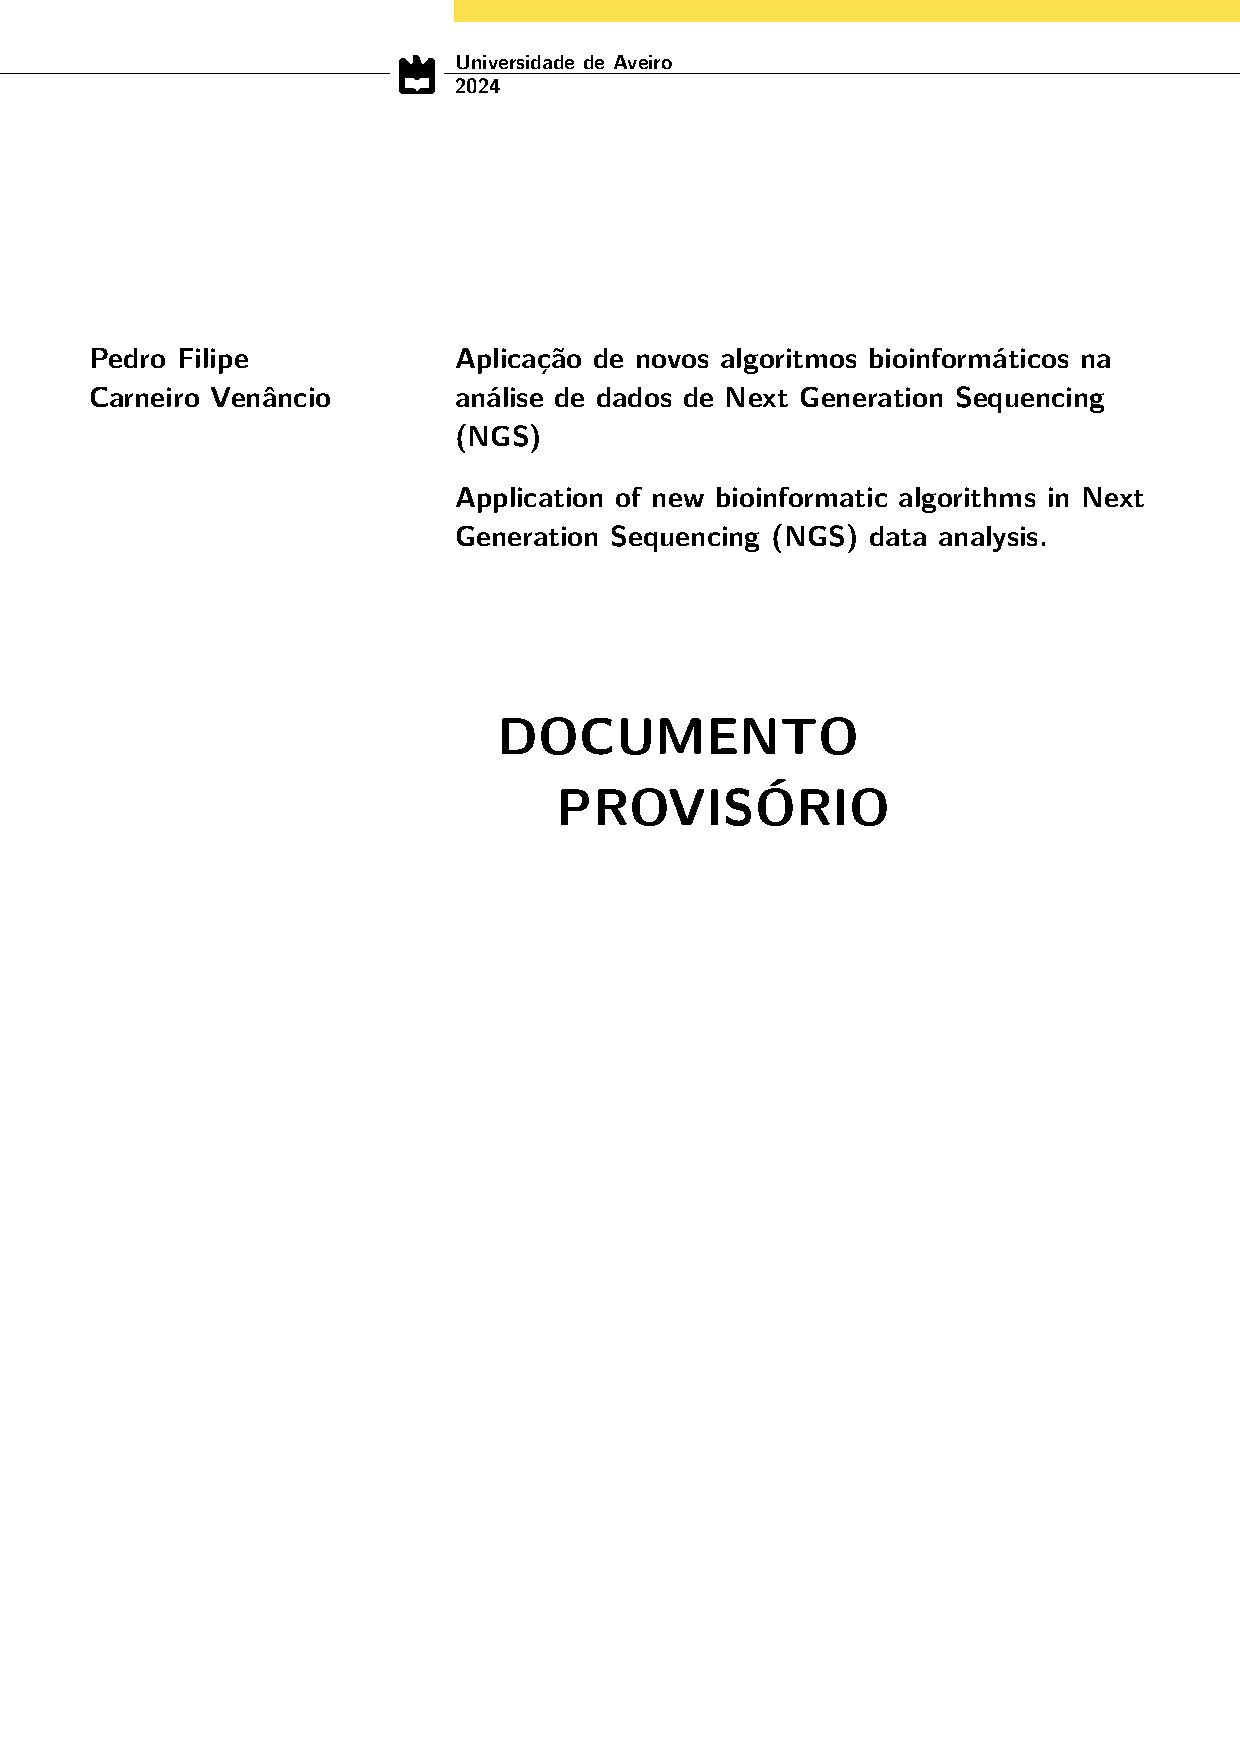
\includepdf[pages=-]{cover.pdf}

% Uncomment to enable English
%\selectlanguage{english}


% Front matter

%Custom Chapter style named `thesis`
\makechapterstyle{thesis}{% Based on ell
  \chapterstyle{default}
  \renewcommand*{\chapnumfont}{\normalfont\sffamily}
  \renewcommand*{\chaptitlefont}{\normalfont\Huge\sffamily}
  \settowidth{\chapindent}{\chapnumfont 111}
  \renewcommand*{\chapterheadstart}{\begingroup
    \vspace*{\beforechapskip}%
    \begin{adjustwidth}{}{-\chapindent}%
    \hrulefill
    \smash{\rule{0.4pt}{15mm}}
    \end{adjustwidth}\endgroup}
  \renewcommand*{\printchaptername}{}
  \renewcommand*{\chapternamenum}{}
  \renewcommand*{\printchapternum}{%
    \begin{adjustwidth}{}{-\chapindent}
    \hfill
    \raisebox{10mm}[0pt][0pt]{\fontsize{30}{25}\selectfont\chapnumfont \thechapter}%
                              \hspace*{1em}
    \end{adjustwidth}\vspace*{-3.0\onelineskip}}
  \renewcommand*{\printchaptertitle}[1]{%
    \vskip\onelineskip
    \raggedleft {\chaptitlefont ##1}\par\nobreak\vskip 4\onelineskip}}


% Select chapter style from existing or select custom
%\chapterstyle{thesis} % Others: dowding, demo2, dash, chappell, brotherton, bianchi, ger, madsen, tatcher, veelo,indexes)
% thesis can also be used as defined previously
% Check the memoir documentation for the available themes
% Default is veelo
\chapterstyle{veelo}
\makeoddfoot{plain}{}{\thepage}{} % Added by André Zúquete to fix a page numbering issue on the veelo chapter style


% If you feel adventurous you can also define all aspects of your theme
% Use either this input or the chapterstyle before
% % Rules
\newcommand{\thinRule}{\rule{\textwidth}{0.25pt}}

% Customize heading appearances
% Define styles
\newcommand{\partSize}{\Huge}
\newcommand{\partStyle}{\lsstyle\scshape}
\newcommand{\chapterSize}{\Huge}
\newcommand{\chapterStyle}{\lsstyle\scshape}
\newcommand{\chapterAfter}{}
\newcommand{\sectionSize}{\Large}
\newcommand{\sectionStyle}{\scshape\MakeTextLowercase}
\newcommand{\subsectionSize}{\large}
\newcommand{\subsectionStyle}{\scshape\MakeTextLowercase}
\newcommand{\subsubsectionSize}{\large}
\newcommand{\subsubsectionStyle}{\scshape\MakeTextLowercase}
\newlength{\partNumSizePt}
\setlength{\partNumSizePt}{60pt}
\newlength{\chapterNumSizePt}
\setlength{\chapterNumSizePt}{60pt}
\newcommand{\partNumSize}{%
  \fontsize{\partNumSizePt}{1.2\partNumSizePt}\selectfont%
}
\newcommand{\partNumStyle}{\partChapterNumColor}
\newcommand{\chapterNumSize}{%
  \fontsize{\chapterNumSizePt}{1.2\chapterNumSizePt}\selectfont%
}
\newcommand{\chapterNumStyle}{\partChapterNumColor}

% Customize parts
\renewcommand{\partnamefont}{\partSize\partStyle}
\renewcommand{\partnumfont}{\partNumSize\partNumStyle}
\renewcommand{\printpartname}{}
\renewcommand{\printparttitle}[1]{%
  \normalfont\normalcolor\partnamefont #1
}

% Customize chapters
\makeatletter
\setlength{\beforechapskip}{30pt}
\renewcommand*{\chapterheadstart}{\vspace*{\beforechapskip}}
\setlength{\afterchapskip}{3ex}
\setlength{\midchapskip}{3ex}
\renewcommand*{\chapnamefont}{%
  \Large\flushright\chapterStyle\partChapterNumColor%
}
\renewcommand*{\chapnumfont}{\chapterNumSize\chapterNumStyle}
\renewcommand*{\chaptitlefont}{%
  \normalfont\flushleft\normalcolor\chapterSize\chapterStyle%
}
\renewcommand*{\printchaptername}{%
  \chapnamefont\MakeTextLowercase{\@chapapp}%
}
\renewcommand*{\chapternamenum}{\quad}
\renewcommand*{\printchapternum}{%
%  \chapnumfont\textls[-75]{\classicstylenums{\thechapter}}%
 \chapnumfont\textls[-75]{\thechapter}%

}
\renewcommand*{\printchaptertitle}[1]{%
  \chaptitlefont #1
  \chapterAfter
}
\makeatother
% Customize sections and subsections
\setsecnumformat{\csname my#1\endcsname\quad}
\setsecheadstyle{\sectionSize\sectionStyle}
\newcommand{\mysection}{{\thesection}}
\setlength{\beforesecskip}{3em}


\setsubsecheadstyle{\subsectionSize\subsectionStyle}
\newcommand{\mysubsection}{{\normalfont\subsectionSize\thesubsection}}
\setlength{\beforesubsecskip}{3em}

\setsubsubsecheadstyle{\subsubsectionSize\subsubsectionStyle}
\newcommand{\mysubsubsection}{{\normalfont\subsubsectionSize\thesubsubsection}}
\setlength{\beforesubsubsecskip}{2em}

% Customize "Table of ..." appearance
% Customize headings
\newcommand{\renewPrintXTitle}[1]{%
  \renewcommand{#1}[1]{%
    \printchaptertitle{##1}%
  }%
}
\renewPrintXTitle{\printtoctitle}
\renewPrintXTitle{\printlottitle}
\renewPrintXTitle{\printloftitle}

% Customize ToC headings
\renewcommand{\cftpartfont}{\partChapterNumColor\partStyle}
\renewcommand{\cftchapterfont}{\chapterStyle}
\renewcommand{\cftsectionfont}{}
\renewcommand{\cftsubsectionfont}{}
\renewcommand{\cftfigurefont}{}
\renewcommand{\cfttablefont}{}
\newcommand{\cftlstlistingfont}{}

% Increase number width
\newlength{\cftNumWidthIncrease}
\setlength{\cftNumWidthIncrease}{0.25em}
\addtolength{\cftpartnumwidth}{\cftNumWidthIncrease}
\addtolength{\cftchapternumwidth}{\cftNumWidthIncrease}
\addtolength{\cftsectionindent}{\cftNumWidthIncrease}
\addtolength{\cftsubsectionindent}{\cftNumWidthIncrease}
% No leader dots
%\renewcommand*{\cftpartdotsep}{\cftnodots}
%\renewcommand*{\cftchapterdotsep}{\cftnodots}
%\renewcommand*{\cftsectiondotsep}{\cftnodots}
%\renewcommand*{\cftsubsectiondotsep}{\cftnodots}
%\renewcommand*{\cftfiguredotsep}{\cftnodots}
%\renewcommand*{\cfttabledotsep}{\cftnodots}
%\newcommand*{\cftlstlistingdotsep}{\cftnodots}
% Set page numbers immediately after entry text
\newcommand{\tocEntryPageSep}{\hspace{1em}}
\renewcommand{\cftpartleader}{\cftdotfill{\cftdotsep}}
%\renewcommand{\cftpartafterpnum}{\cftparfillskip}
%\renewcommand{\cftchapterleader}{\tocEntryPageSep}
\renewcommand{\cftchapterleader}{\cftdotfill{\cftdotsep}}
%\renewcommand{\cftchapterafterpnum}{\cftparfillskip}
\renewcommand{\cftsectionleader}{\cftdotfill{\cftdotsep}}
%\renewcommand{\cftsectionafterpnum}{\cftparfillskip}
\renewcommand{\cftsubsectionleader}{\cftdotfill{\cftdotsep}}
%\renewcommand{\cftsubsectionafterpnum}{\cftparfillskip}
\renewcommand{\cftfigureleader}{\cftdotfill{\cftdotsep}}
%\renewcommand{\cftfigureafterpnum}{\cftparfillskip}
\renewcommand{\cfttableleader}{\cftdotfill{\cftdotsep}}
%\renewcommand{\cfttableafterpnum}{\cftparfillskip}
\newcommand{\cftlstlistingleader}{\cftdotfill{\cftdotsep}}
%\newcommand{\cftlstlistingafterpnum}{\cftparfillskip}
% Customize page numbers
\newcommand{\tocPageStyle}{\tocPageColor}
\renewcommand{\cftpartpagefont}{\tocPageStyle}
\renewcommand{\cftchapterpagefont}{\tocPageStyle}
\renewcommand{\cftsectionpagefont}{\tocPageStyle}
\renewcommand{\cftsubsectionpagefont}{\tocPageStyle}
\renewcommand{\cftfigurepagefont}{\tocPageStyle}
\renewcommand{\cfttablepagefont}{\tocPageStyle}
\newcommand{\cftlstlistingpagefont}{\tocPageStyle}

% Abstract
% Remove indents around abstract text
\setlength{\absleftindent}{0pt}
\setlength{\absrightindent}{0pt}
% Change font size to conform with the rest of the document text
\renewcommand{\abstracttextfont}{\normalsize}

% Customize headers and footers including page numbers
\newcommand{\hfTextSize}{\footnotesize}
\newcommand{\headTextStyle}{\lsstyle\scshape\MakeTextLowercase}
\nouppercaseheads
\makeevenhead{headings}%
             {\hfTextSize\thepage}%
             {}%
             {\hfTextSize\headTextStyle\leftmark}
\makeevenhead{plain}%
             {\hfTextSize\thepage}%
             {}%
             {\hfTextSize\headTextStyle\leftmark}
\makeoddhead{headings}%
            {\hfTextSize\headTextStyle\rightmark}%
            {}%
            {\hfTextSize\thepage}
\makeoddhead{plain}%
            {\hfTextSize\headTextStyle\rightmark}%
            {}%
            {\hfTextSize\thepage}


% Customize captions
\newcommand{\captionSize}{\small}
\newcommand{\captionStyle}{\scshape}
\newcommand{\captionWidthRatio}{0.9}

\captionnamefont{\captionSize\captionStyle}
\captiontitlefont{\captionSize}
\captiondelim{ -- }
\captiontitlefinal{}
\changecaptionwidth
%\captionwidth{\captionWidthRatio\textwidth}

% Define colors
%\newcommand{\titleColor}{\color[rgb]{0.616, 0.0627, 0.176}}
\newcommand{\titleColor}{\color[rgb]{0,0,0}}

\newcommand{\partChapterNumColor}{\titleColor}
\newcommand{\dropCapColor}{\titleColor}
%\newcommand{\tocPageColor}{\color[rgb]{0.0980, 0.329, 0.651}}

\newcommand{\tocPageColor}{\color[rgb]{0, 0,0}}
\definecolor{shade0}{rgb}{1.0 , 1.0 , 1.0 }
\definecolor{shade1}{rgb}{0.9 , 0.9 , 0.9 }
\definecolor{shade2}{rgb}{0.8 , 0.8 , 0.8 }
\definecolor{shade3}{rgb}{0.65, 0.65, 0.65}
\definecolor{shade4}{rgb}{0.45, 0.45, 0.45}
\definecolor{shade5}{rgb}{0.0 , 0.0 , 0.0 }



%Exclude sub figures from List of Figures
%\captionsetup[subfloat]{list=no}

% Texts
\newenvironment{introduction}
{%
  \begin{minipage}{\textwidth}%
   \itshape%
}
{%
  \end{minipage}%
  \par\addvspace{2\baselineskip plus 0.2\baselineskip minus 0.2\baselineskip}%
}

% Select Page style
\pagestyle{plain}


\frontmatter

\tightlists
\midsloppy
\raggedbottom

\setcounter{tocdepth}{2} %subsections are added to the TOC
\setcounter{secnumdepth}{4} %subsubsections are numbered

% Initial document tables start here: TOC, LOF, LOT, Glossary
% Table of contents with slightly smaller font
\cleardoublepage
{\small\tableofcontents}

% List of figures with slightly smaller font
\cleardoublepage
{\small\listoffigures}

% List of tables with slightly smaller font
\cleardoublepage
{\small\listoftables}

% List of code snippets

% Fix for Listings with memoir

\RenewDocumentCommand \chapter { s O{#3} m }{%
  \FloatBarrier
  \IfValueTF{#1}  % if optional star is seen
    {\oldchapter*{#2}}
    {\oldchapter#1{#2}}
}

\renewcommand{\listingscaption}{Código}
\renewcommand{\listoflistingscaption}{Lista de Excertos de Código}
\cleardoublepage
{\small\listoflistings}
\addcontentsline{toc}{chapter}{\listoflistingscaption}

% Reset Chapters
\renewcommand{\chapter}[2][]{
  \FloatBarrier
  \oldchapter#1{#2}
}

% Print Glossary
{\small\chapter{Glossary}

\footnotesize
\SingleSpacing

\begin{multicols}{2}
\begin{acronym}[AAAAAA]

	\acro{ngs}[NGS]{Next Generation Sequencing}
	\acro{clia}[CLIA]{Clinical Laboratory Improvement Amendments}
	\acro{iso}[ISO]{International Organization for Standardization}
	\acro{wes}[WES]{Whole Exome Sequencing}
	\acro{wgs}[WES]{Whole Genome Sequencing}
	\acro{acgh}[aCGH]{Comparative Genomic Hybridization}
	\acro{fish}[FISH]{Fluorescence In Situ Hybridization}
	\acro{qf-pcr}[QF-PCR]{full name}
	\acro{qpcr}[qPCR]{full name}
	\acro{rt-pcr}[RT-PCR]{full name}
	\acro{mlpa}[MLPA]{Multiplex Ligation-Dependent Probe Amplification}
	\acro{nipt}[NIPT]{Non-Invasive Prenatal Testing}
	\acro{dna}[DNA]{Deoxyribonucleic Acid}
	\acro{hgp}[HGP]{Human Genome Project}
	\acro{crisp}[CRISPR]{full name}
	\acro{crispr-cas9}[CRISPR-Cas9]{full name}
	\acro{rna}[RNA]{Ribonucleic Acid}
	\acro{a}[A]{Adenine}
	\acro{t}[T]{Thymine}
	\acro{c}[C]{Cytosine}
	\acro{g}[G]{Guanine}
	\acro{SWOT}[SWOT]{Strengths Weeknesses Opportunities and Threats}
	\acro{wsl}[WSL]{Windows Subsystem for Linux}
	\acro{es}[ES]{Exome Sequencing}
	\acro{gs}[GS]{Genome Sequencing}
	\acro{hg38}[GRCh38/hg38]{Reference Consortium Human Build 38}
	\acro{bam}[BAM]{Binary Alignment Map}
	\acro{sam}[SAM]{Sequence Alignment Map}
	\acro{cram}[CRAM]{Compressed Reference-oriented Alignment Map}
	\acro{vus}[VUS]{Variants With Unknown Significance}
	\acro{nlp}[NLP]{Natural Language Processing}
	\acro{snps}[SNPs]{Single-Nucleotide Polymorphisms}
	\acro{snvs}[SNVs]{Single-Nucleotide Variants}
	\acro{indels}[INDELs]{Insertions and Deletions}
	\acro{cnvs}[CNVs]{Copy Number Variants}
	\acro{vaf}[VAF]{Variant Allele Frequency}
	\acro{ref}[REF]{Reference Allele}
	\acro{alt}[ALT]{Alternate Allele}
	\acro{gq}[GQ]{Genotype Quality}
	\acro{vcf}[VCF]{Variant Call Format}
	\acro{gvcf}[gVCF]{Genomics Variant Call Format}
	\acro{maf}[MAF]{Mutation Annotation Format}
	\acro{bed}[BED]{Browser Extensible Data}
	\acro{csv}[CSV]{Comma-Separated Values}
	\acro{pdf}[PDF]{Portable Document Format}
	\acro{gdpr}[GDPR]{General Data Protection Regulation}
	\acro{fr}[FR]{Functional Requirements}
	\acro{nfr}[NFR]{Non-Functional Requirements}
	\acro{mane}[MANE]{Matched Annotation from NCBI and EMBL-EBI}
	\acro{gui}[GUI]{Graphical User Interface}
	\acro{bp}[BP]{Base Pair}


\end{acronym}
\end{multicols}

}

%%%%%%%%%%%%%%%%%%%%%%%%%%%%%%%%%%%%%%%%%%%%%%%%%%%%%%%
% Main document starts here
%%%%%%%%%%%%%%%%%%%%%%%%%%%%%%%%%%%%%%%%%%%%%%%%%%%%%%%

\mainmatter

% Line spacing: 1.5 pt 
\OnehalfSpacing

%%%%%%%%%%%%%%%%%%%%%%%%%%%%%%%%%%%%%%%%%%%%%%%%%%%%%%%
% Start of Thesis text 
%%%%%%%%%%%%%%%%%%%%%%%%%%%%%%%%%%%%%%%%%%%%%%%%%%%%%%%

% Uncomment to add further chapters
\chapter{Introdução}
\label{chapter:introduction}

\begin{introduction}
A short description of the chapter.

A memorable quote can also be used.
\end{introduction}



\section{Acrónimos}

Primeira e seguintes referências: \ac{h2o}, \ac{h2o}

Plural, acrónimo expandido e curto: \acp{h2o}, \acl{h2o}, \acs{h2o}

Com citação\footnote{Necessária entrada na bibliografia}: \ac{adsl}, \ac{adsl}


\section{Fontes}

\begin{itemize}
\item{\tiny Tiny}
\item{\scriptsize Scriptsize}
\item{\footnotesize Footnotes}
\item{\small Small}
\item{\normalsize Normal}
\item{\large large}
\item{\Large Large}
\item{\LARGE LARGE}
\item{\huge huge}
\item{\Huge Huge}
\end{itemize}

\section{Unidades}

Utilizando o pacote \verb|siunitx| é possível utilizar unidades do Sistema Internacional. Exemplo: a aceleração da gravidade é de \SI{9.8}{\metre\per\second\squared} e um ficheiro ocupa \SI{1}{\mebi\byte}. 

\section{Code Blocks}
%\lipsum[5]
Uma listagem pode ser apresentada com o ambiente \texttt{listing}, que é um float (objeto flutuante, tal como uma figura ou uma tabela).

A listagem em Código~\ref{lbl:snippet-test} mostra um exemplo em C.

\begin{listing}[h]
\begin{minted}{c}

#include <stdio.h>
#define N 10
/* Block
 * comment */
 
int main()
{
    int i;
 
    // Line comment.
    puts("Hello world!");
 
    for (i = 0; i < N; i++)
    {
        puts("LaTeX is also great for programmers!");
    }
 
    return 0;
}
\end{minted}
\caption{This caption appears below the code.}
\label{lbl:snippet-test}
\end{listing}

%\lipsum[5]

\section{Citações}

Algumas formas distintas de citar:

\begin{itemize}
    \item \textbf{Apenas referência}:~\cite{rfc44}
    \item \textbf{Apenas data}:~\citedate{rfc44}
    \item \textbf{Apenas ano}:~\citeyear{rfc44}
    \item \textbf{Apenas autor}:~\citeauthor{rfc44}
    \item \textbf{Apenas editor}:\citelist{rfc44}{organization}
    \item \textbf{Autor e referência}:\citet{rfc44}
\end{itemize}

%\chapter{Software development process}
\label{chapter:Analysis tool}

\begin{introduction}
    "The only source of knowledge is experience." - Albert Einstein
\end{introduction}

\section{Analysis}

\section{Planning}

\section{Design}


\section{Development}
\subsection{Environment preparation }
\subsubsection{\textbf{Windows Subsystem for Linux (WSL)}}

On Windows, developers have access to both the Windows and Linux environments, thanks to the Windows Subsystem for Linux (WSL). With WSL, it is possible to install different Linux distributions, such as Ubuntu, OpenSUSE, Kali, Debian, Arch Linux, among others. This allows Linux applications, utilities and command-line tools to be used directly in Windows, without the need to modify the operating system, resort to virtual machines or dual boot. 

In the context of the development of this tool, the need to install WSL was driven mainly due to the scenario in which many essential tools and software for bioinformatics are designed to work in Linux environments. For this reason, we followed the set of steps recommended on the Microsoft website to configure this environment (Build 19041 or higher). \cite{wsl}

\subsubsection{\textbf{Anaconda and Conda}}

After installing WSL, the installation step of Anaconda followed, a platform for data science in Python/R that includes conda, a package and environment manager, making it easier for users to manage a collection of more than 7,500 open source packages. \cite{anaconda1}

In the case of the creation of the metrics analysis tool, this step was fundamental to allow the installation and maintenance of all the packages and dependencies necessary for the operation of the software. By creating a conda environment, it was possible to ensure that all installed tools work independently without conflicts between versions and packages, thus ensuring the reproducibility of the created software. \cite{anaconda2}

Following the documentation provided by Anaconda, the installation and creation of the conda environment was carried out. \cite{anaconda3} 

Additionally, all the dependencies of the attached x-list were installed within the created environment. This installation was carried out by installing package by package, however, an environment.yaml file was made available that allows the bulk installation \cite{anaconda4} of all dependencies on the versions compatible with the software.

\subsubsection{\textbf{Git and GitHub}}

GitHub is a platform that allows users to store, share, and collaborate on code writing with others.

Its operation is based on repositories managed by Git, a version control system that tracks all changes made by one or more users in a project.

When files are uploaded to GitHub, they become part of the created repository. Any change (commit) to any file is automatically tracked. These changes, made locally, are usually synchronized continuously by pushing the committed changes. Similarly, any changes made locally by another user and synchronized on GitHub can be retrieved by making a pull request.

Thus, by using the documentation of Git and GitHub, this practice was implemented, which not only ensures that each version of the created software is recorded—guaranteeing that the work is not lost and allowing for version rollback in case of bugs—but also ensures that all software produced is reproducible and available for deployment by any user. \cite{github}


\subsubsection{\textbf{SAMtools}}

SAMtools is an essential tool for the manipulation and analysis of DNA sequencing data. First released in 2009, it allows for converting, manipulating, sorting, querying, calculating statistics, calling variants, and analyzing sequencing data in SAM, BAM, and CRAM formats.

Among the many functionalities of SAMtools, the most notable are its ability to convert formats, manipulate and index files, visualize and export data, and calculate statistics, such as "depth," which served as the basis for the tool created. \cite{samtools}

In this case, a Python function was developed to generate a .depth file with the desired metrics, using SAMtools depth.

\begin{listing}[h]
\begin{minted}{python}
import subprocess

def depth(bam_path, bed_path, depth_path, gene_selection=None, exon_selection=None): 
    """ 
    Calculate the depth of coverage for specific exons of genes in a BAM file using samtools.
s
    Args: 
        bam_path (str): Path to the BAM file.
        bed_path (str): Path to the Universal BED file containing exon coordinates.
        depth_path (str): Path to save the depth output.
        gene_selection (list or None): List of gene names to include in the depth calculation. 
                                       If None, all genes will be included.
        exon_selection (list or None): List of exon numbers to include in the depth calculation. 
                                       If None, all exons will be included.

    Returns: 
        None
    """ 
    
    gene_filter = ','.join(map(str, gene_selection)) if gene_selection else '' 
    exon_filter = ','.join(map(str, exon_selection)) if exon_selection else ''
    
    # Construct awk command to filter based on gene and exon selection
    awk_command = (f'awk -v gene_filter={gene_filter} -v exon_filter={exon_filter} '
                   f'\'{{split(exon_filter, arr, ","); '
                   f'if (($4 == gene_filter || gene_filter == "") && '
                   f'("" in arr || $5 == arr[1])) {{sub(/^chr/, "", $1); print}}}}\' {bed_path}')
    
    # Construct samtools command to calculate depth
    samtools_command = f'samtools depth -b - {bam_path} > {depth_path}'
    
    # Run the commands using subprocess
    try:
        subprocess.run(f'{awk_command} | {samtools_command}', shell=True, check=True)
    except subprocess.CalledProcessError as e:
        print(f"Error occurred: {e}")
\end{minted}
\caption{Python function to calculate depth of coverage using samtools and awk.}
\label{lbl:snippet-test}
\end{listing}


\section{Testing and validation}


\section{Optimization}


\section{Deployment}


\section{Documentation}


\section{Maintenance}
%\chapter{Results}
\label{chapter:Results}

\begin{introduction}
    "The only source of knowledge is experience." - Albert Einstein
\end{introduction}

\section{Evolution of Software Development}

The software development process has undergone several important stages, each enhancing its functionality and usability. The figures below illustrate the application's progress, showcasing different phases of refinement as the project matured.

\subsection{Initial Stages: Basic Functionality and User Interaction}

The first figure (Figure \ref{fig:v1}) represents the early stages of development, where the primary focus was on creating a user-friendly interface for calculating average read depth and coverage metrics from a BAM file for a Single Gene. In this version, the application prominently features a two-step process where the user selects a BED file releated to de gene to analyse and one or more BAM files. These files are then processed to calculate key metrics, which are displayed in the results table below. This simple design allowed for efficient user interaction but was somewhat limited in terms of flexibility and scope.

At this stage, the core challenge was to ensure that the software could handle large genomic files while presenting the results in a clear and intuitive format. The layout emphasizes simplicity, making it easier for users to navigate through the two-step process. However, as the project progressed, the need for more advanced features became evident.

\begin{figure}[H]
    \centering
    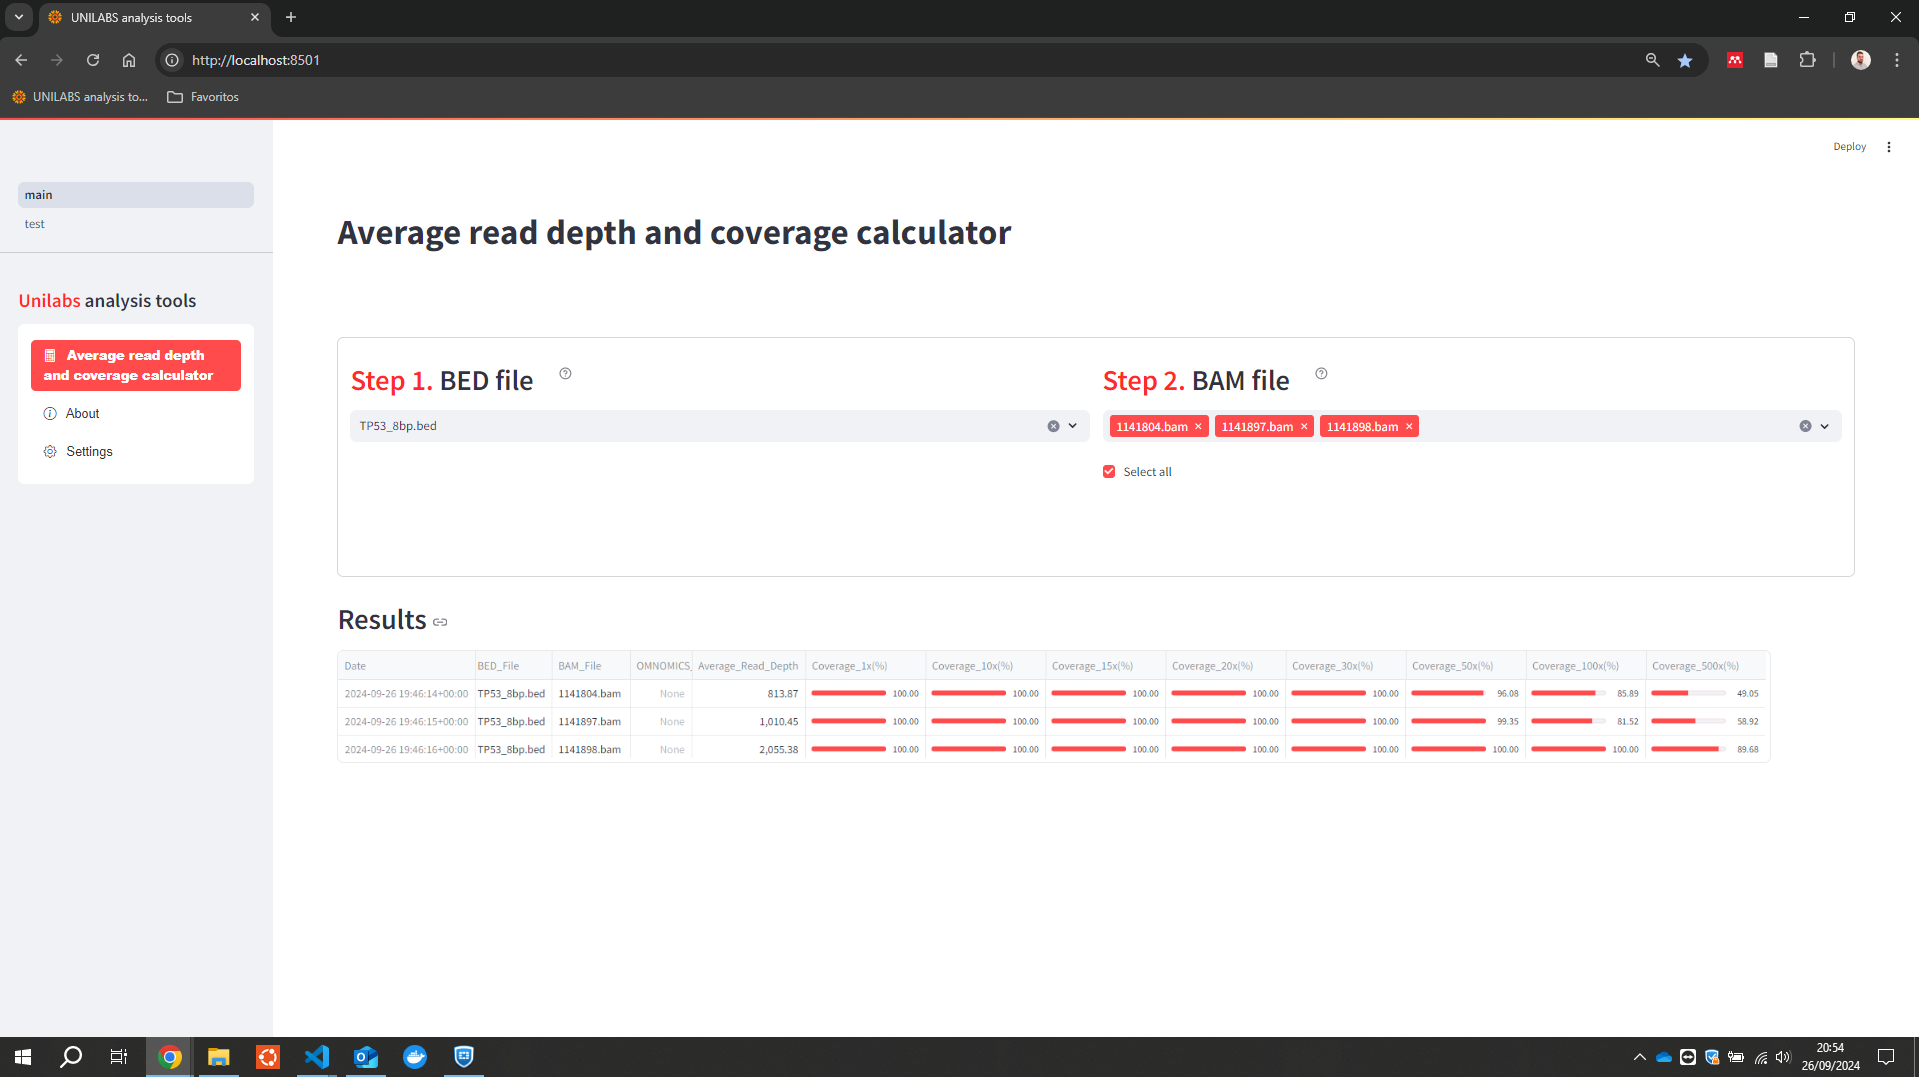
\includegraphics[width=1\textwidth]{figs/v1.png}
    \caption{First version of the GUI.} 
    \label{fig:v1}
\end{figure}

\subsection{Refinement: Introducing Flexibility and Multiple Analysis Modes}

In the second figure (Figure \ref{fig:v2}), the software has significantly evolved to include more detailed analysis options. The interface now presents multiple analysis types: \textit{Single Gene}, \textit{Gene Panel}, and \textit{Exome}, catering to different research needs. This flexibility represents a major shift from the earlier version, as it now allows users to select specific genome assemblies and regions of interest by using an universal BED file. Additionally, the results section has been split into tabs such as \textit{Overview} and \textit{Exon Details}, giving users the ability to drill down into the metrics for a single gene or explore exon-level coverage details. However, even though this last features were thinked to be used in this version, they only have been work fully in the last version of the software. 

\begin{figure}[H]
    \centering
    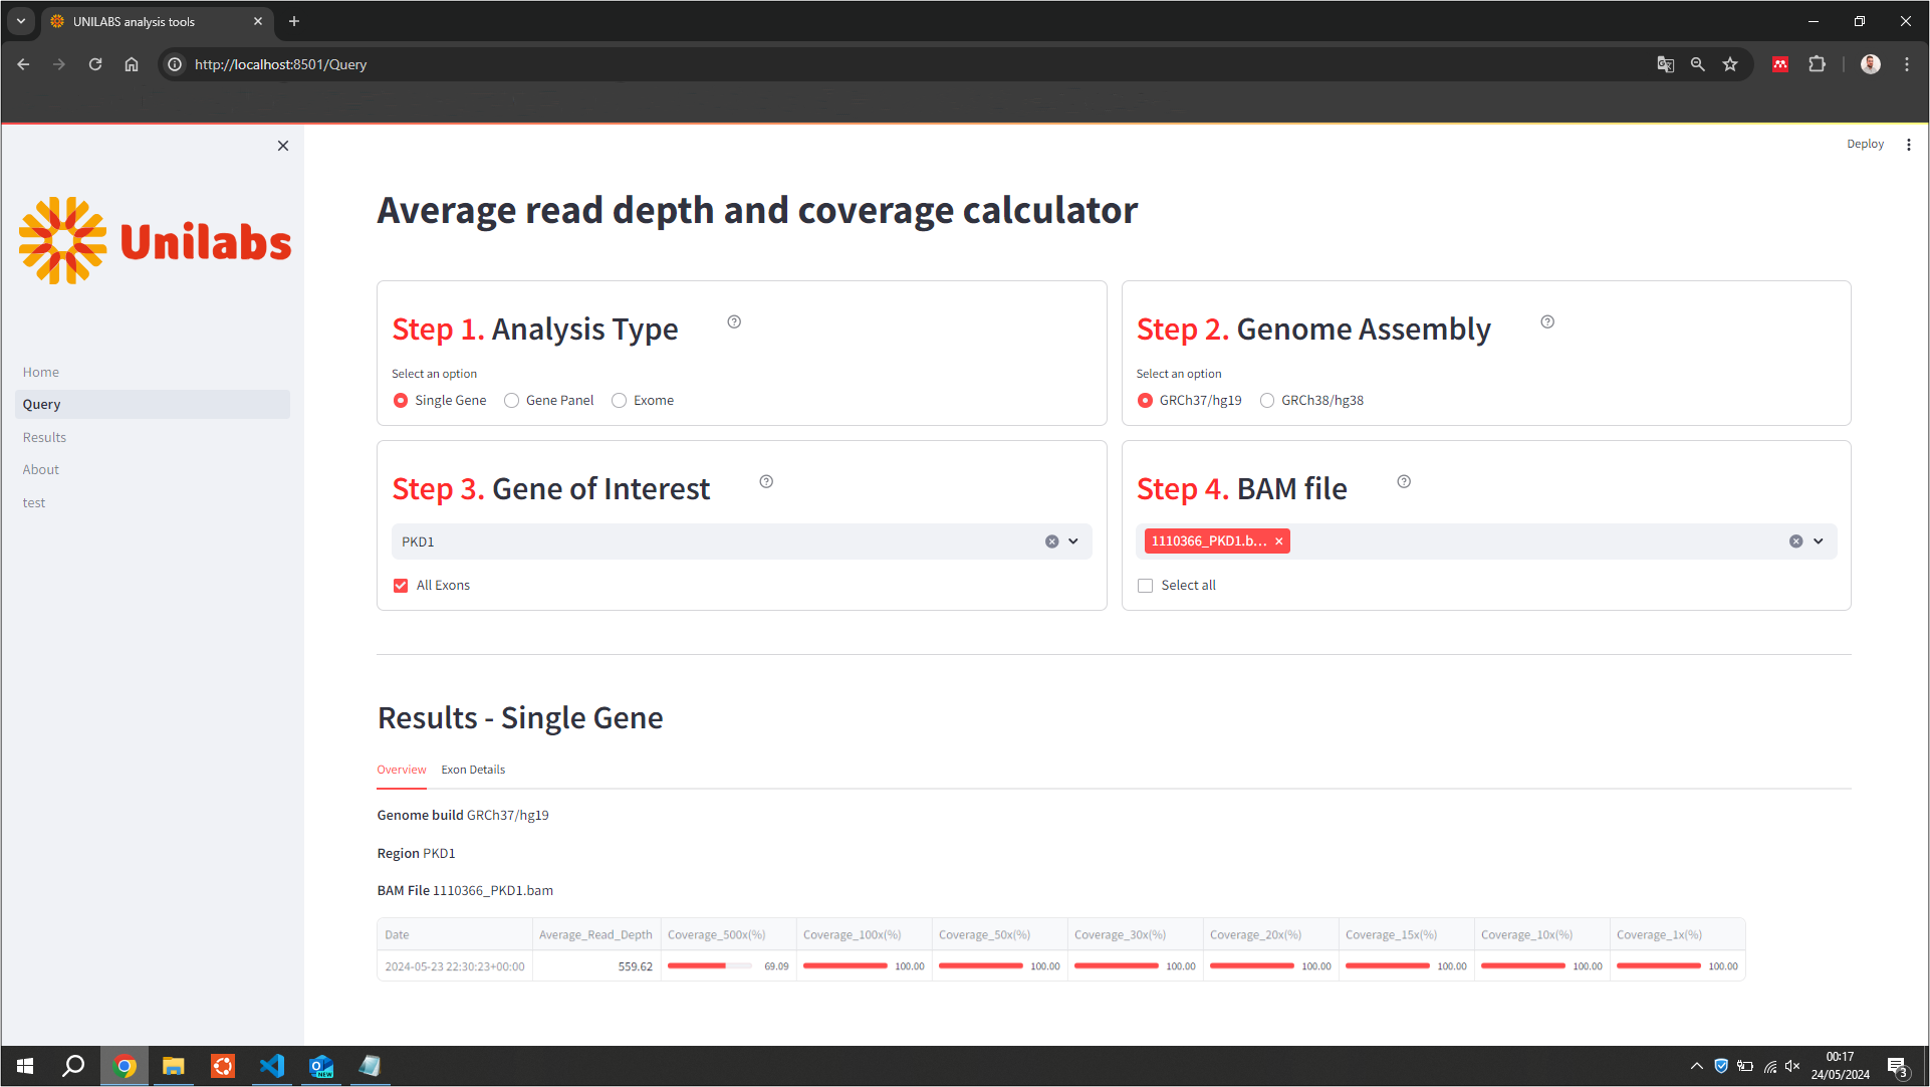
\includegraphics[width=1\textwidth]{figs/v2.png}
    \caption{Second version of the GUI.} 
    \label{fig:v2}
\end{figure}






\section{Real data test running}
\section{Test and validation}

De forma a validar a ferramenta, foram realizados testes com dados reais de sequenciação genómica. Os resultados obtidos foram comparados com os obtidos por outras ferramentas de análise de dados genómicos comerciais, como a \textit{Omnomics}. Foram reproduzidas as análises para Singles Gene e Gene Panel. 
No primeiro caso, para o mesmo ficheiro de alinhamento .bam, e usando como referência a mesma versaão do genoma humano (hg19), os resultados obtidos foram semelhantes como se pode observar na Figura

\section{Performance}


\section{Comparison with other tools}


\section{Users feedback}







%\chapter{Additional activities during the internship}
\label{chapter:Additional activities during the internship}

\begin{introduction}
    "The only source of knowledge is experience." - Albert Einstein
\end{introduction}


\section{Additional Activities during the Internship}

As part of the internship, an additional activity involved the development of a gene panel creation tool. The purpose of the tool is to streamline the creation and management of gene panels, which are commonly used in genomic analyses.

The gene panel creator allows the user to define a panel by specifying a name and providing a list of genes. The user can paste the list of genes into the designated field, and the tool processes this input to create a gene panel. Once created, the panel becomes available within the system for further use in various analyses.

An additional feature of the tool is the generation of a BED file containing the genomic coordinates of the genes included in the panel. This file can be downloaded directly from the tool's interface, ensuring that the user has access to the relevant genomic regions for further study. The BED file is automatically verified to ensure that all genes are correctly recognized by the system before it is made available for download.

This gene panel creation tool was developed to improve the efficiency of handling gene panels, reducing the manual workload typically involved in their curation and preparation for analysis. The ability to automatically generate and download BED files associated with specific gene panels has proven to be a valuable addition to the software's functionality, ultimately benefiting the genomic analysis workflows at Unilabs.

\begin{figure}[H]
    \centering
    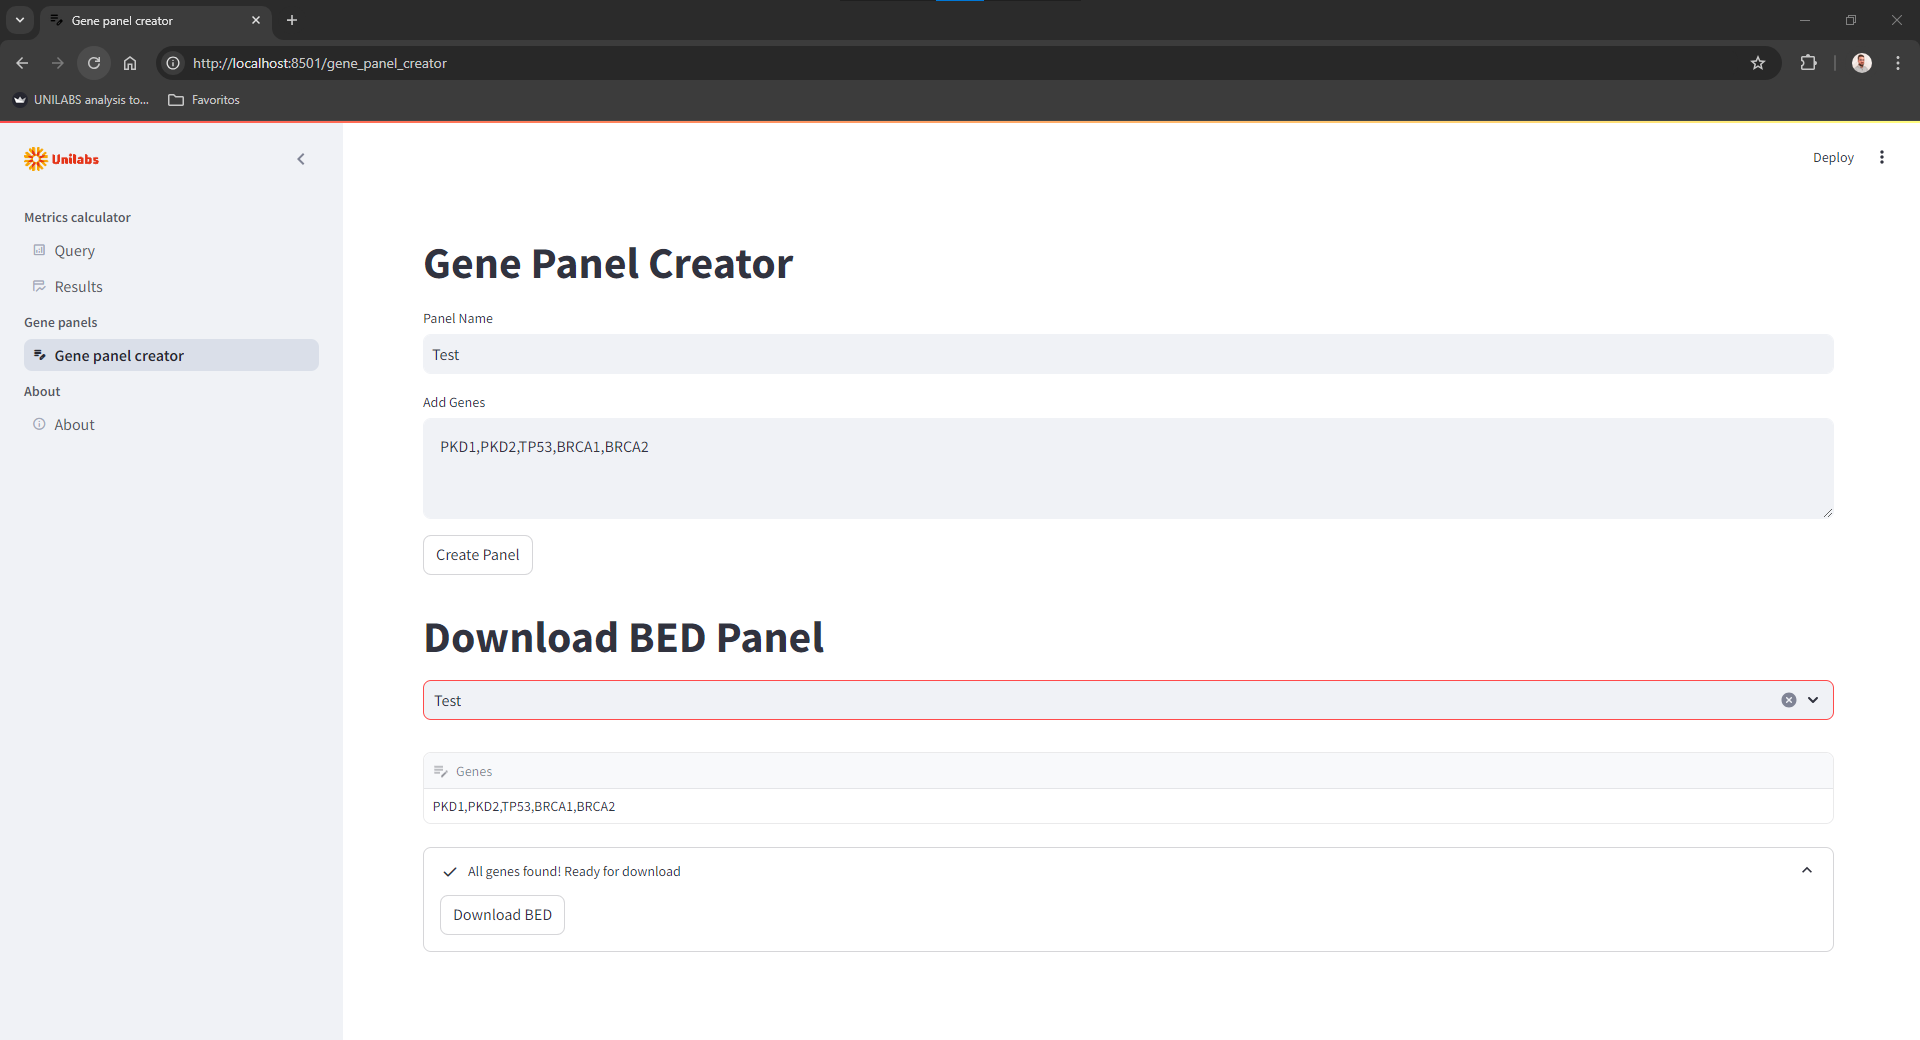
\includegraphics[width=\textwidth]{figs/v3.13.png}
    \caption{Gene Panel Creator Interface}
    \label{fig:gene_panel_creator}
\end{figure}


%%%%%%%%%%%%%%%%%%%%%%%%%%%%%%%%%%%%%%%%%%%%%%%%%%%%%%%
% End of Thesis text 
%%%%%%%%%%%%%%%%%%%%%%%%%%%%%%%%%%%%%%%%%%%%%%%%%%%%%%%

\backmatter

%%%%%%%%%%%%%%%%%%%%%%%%%%%%%%%%%%%%%%%%%%%%%%%%%%%%%%%
% Print all used references
%%%%%%%%%%%%%%%%%%%%%%%%%%%%%%%%%%%%%%%%%%%%%%%%%%%%%%%

\begingroup
\renewcommand{\bibfont}{\footnotesize}
% Redefine References name to Portuguese
% Change if you are using english
\defbibheading{bibliography}[Referências]{
	\chapter{#1}
}
\SingleSpacing
\setlength\bibitemsep{8pt}
\printbibliography[heading=bibliography]
\endgroup


%%%%%%%%%%%%%%%%%%%%%%%%%%%%%%%%%%%%%%%%%%%%%%%%%%%%%%%
% Load appendix
%%%%%%%%%%%%%%%%%%%%%%%%%%%%%%%%%%%%%%%%%%%%%%%%%%%%%%%

\mainmatterWithoutReset
\appendix

\chapter{Additional content}


\end{document}
